\documentclass[a4paper]{article}
\usepackage[utf8]{inputenc}
\usepackage[natbib,sorting=none]{biblatex}
\usepackage{graphicx}
\usepackage{acronym}
\usepackage{indentfirst}
\usepackage{requirements} % custom package
\usepackage[htt]{hyphenat}
\usepackage{fancyhdr}
\usepackage{enumitem}
\usepackage{listings}
\usepackage{xcolor}
\usepackage{pifont}

\newcommand{\requirement}{\ding{229}}%
\definecolor{commentgreen}{RGB}{2,112,10}
\definecolor{eminence}{RGB}{108,48,130}
\definecolor{weborange}{RGB}{255,165,0}
\definecolor{frenchplum}{RGB}{129,20,83}

\addbibresource{references.bib}
\newcommand{\comment}[1]{\textbf{[Comment: #1]}}

\begin{document}
\setlist[enumerate]{label=\alph*),leftmargin=0.4cm, topsep=0cm}
\setlist[itemize]{leftmargin=0.4cm, topsep=0cm}
\begin{figure}[!h]
	\centering
	
\includegraphics[width=80mm]{images/poli-logo.png}
\end{figure}
\hfill
\begin{center}
    \fontsize{18px}{6mm}\selectfont \textsc{\textbf{Software Engineering II project}}
\end{center}
\begin{center}
    \fontsize{12px}{4mm}\selectfont \textsc{Academic Year: 2018/2019}
\end{center}
\hfill
\hfill
\begin{figure}[!h]
	\centering
	
\includegraphics[width=120mm]{images/trackme-logo.png}
\end{figure}
\hfill
\hfill
\begin{center}
    \fontsize{22px}{8mm}\selectfont \textsc{\textbf{Requirement Analysis and\\ Specification Document}}
\end{center}
\begin{center}
    \fontsize{14px}{4mm}\selectfont \textsc{{Draft Version 0.1 - 11/10/2018}}
\end{center}
\hfill
\hfill
\begin{center}
\fontsize{14px}{4mm}\selectfont \textsc{\textit{Davide Rutigliano -  903616}}
\end{center}

\begin{center}
\fontsize{14px}{4mm}\selectfont \textsc{\textit{Claudio Ferrante - 903417\\}}
\end{center}

\begin{center}
\fontsize{14px}{4mm}\selectfont \textsc{\textit{Davide Matta - 903616}}
\end{center}
\pagenumbering{roman}
\tableofcontents
\addcontentsline{toc}{subsection}{Use Cases Summary}
\renewcommand\listtablename{Use Cases Summary}
\listoftables
\addcontentsline{toc}{subsection}{UML Diagrams List}
\renewcommand\listfigurename{UML Diagrams List}
\listoffigures
\rfoot{
\includegraphics[width=30mm]{Images/trackme-logo-mini.png}}
%%%%%%%%%%%%%%%%%%%%%%%%%%%%%%%%%%%%%%%%%%%%%%%%%%%%%%%%%%%%%%
\pagestyle{fancy}
\pagenumbering{arabic}
\newpage
\section{Introduction}

    \subsection{Purpose}
    This Requirement Analysis and Specification Document \cite{ieee1998ieee} is aimed at modeling and describing the system itself, its requirements, its constraints, its components and how it interacts with the world and the users. Moreover, this specifications also addresses some relevant QoS characteristics that the system should guarantee. 
        
    This document is directed and highly recommended to software designers and developers interested in the design and deployment of the proposed system.
    
    \subsection{Scope and Audience}
        \subsubsection{Description of the given problem}
        \textit{TrackMe} is a company that wants to develop an ease of use health monitoring application which offers different services for both young and old people who needs to keep track of their personal data in order to to keep their health safe.
        
        The system should provide an efficient data acquisition facility which gives the possibility to verified \textit{third-party} signed onto the service to request health status information about subscribed customers. The application may also allow \textit{individual} users to connect \textit{external devices} such as smart-watches or similar, to perform a more detailed data acquisition and monitoring.
        
        In addition, the \textit{third-party} may also provide a personalized and non intrusive SOS service for elderly people who requested it.
    
        Moreover, through the \textit{Track4Run} service, \textit{TrackMe} wants to provide to users signed in the application to create a new run: a competition in which other individuals can either participate as \textit{athletes} or watch as \textit{spectators}. Additionally, this feature may exploits other service functionality for keeping track of athletes progresses and for helping them to prevent major accident happen during the run.
        
        \subsubsection{World, Machine and Phenomena}
        
        This section is intended to provide a full description of the proposed system by meaning of \textit{Domains} and \textit{Phenomena} \cite{zave1997four}.
    
        The \textit{Machine Domain} is the set of phenomena that the machine can control: data structures, algorithms, devices and inputs it can get from the world.
        
        In contrast, the \textit{World Domain} is the real-life context in which the \textit{Machine} will be introduced. This is the part of the real-world in which the \textit{Machine} actions will be observed.
        
        The World and the Machine are connected too, because the latter should interact with the first one: this interaction is done through \textit{Shared Domain}, whose phenomena are observable both by the Machine and by the World. Shared Phenomena include events in the real world that the Machine can directly sense and actions in the real world that the Machine can directly cause.
        \newpage
        \begin{table}[!htpb]
        \centering
        \begin{tabular}{|l|l|l|l|}
        \hline
         \textbf{Phenomenon} & \textbf{World} & \textbf{Machine} & \textbf{Shared}\\ \hline
         Registration/Login/Log-out & & & X \\ \hline
         Manage Profile/Change Credentials & & & X \\ \hline
         Application logic & & X & \\ \hline
         Accept/Reject/Send Request & & & X \\ \hline
         Data Subscription/Synchronization & & & X \\ \hline
         Database Query & & X & \\ \hline
         Connect External Device & & & X \\ \hline
         GPS Tracking & & & X \\ \hline
         Enable Sos & & & X \\ \hline
         Locate nearest Ambulance & & & X \\ \hline
         Accident & X & & \\ \hline
         Create/Delete/Enroll/Watch/Start Run & & & X \\ \hline
        \end{tabular}
        \end{table}
        
        \subsubsection{Goals}
        
        \begin{description}
            \item[GOAL-01] Allow a guest to register as an Individual.
            \item[GOAL-02] Allow a guest to register as an Third-Party.
            \item[GOAL-03] The guest should be able to sign in into the application.
            \item[GOAL-04] The user should be able to change his username.
            \item[GOAL-05] The user should be able to change his password.
            \item[GOAL-06] The user should be able to log-out from the system.
            \item[GOAL-07] The individual should be able to change his personal data.
            \item[GOAL-08] The Third-Party should be able to change his organization data.
            \item[GOAL-09] The Third-Party should be able to send requests to the individuals
            \item[GOAL-10] The Third-Party should be able to make group requests.
            \item[GOAL-11] The Third-Party should be able to subscribe to new data, once an Individual request is made.
            \item[GOAL-12] The Individual should be able to accept or reject a request coming from a Third-Party.
            \item[GOAL-13] The Individual shall be able connect an external device to the system.
            \item[GOAL-14] The Third-Party shall be able to activate Automated-SOS service.
            \item[GOAL-15] The Individual shall be able to activate Automated-SOS service.
            \item[GOAL-16] The Dispatcher shall be able to assign an ambulance to an incident.
            \item[GOAL-17] The Organizer shall be able to create a run.
            \item[GOAL-18] The Organizer should be able to start a run.
            \item[GOAL-19] The Organizer should be able to delete a run.
            \item[GOAL-20] The Athlete should be able to enroll a run.
            \item[GOAL-21] The Athlete should be able to unroll a run
            \item[GOAL-22] The Spectator should be able to watch a run.
        \end{description}
    
    \subsection{Document Overview}
        This initial part of the document is intended to provide both an overview of the problem and an idea of the proposed solution.
        
        Following section is aimed at giving a more detailed description of the proposed system, by meaning of the application point of view. Additionally, it addresses functionality, user characteristics, dependencies and constraints.
        
        Third chapter shows a detailed analysis of \textit{TrackMe} in terms both functional and non-functional requirements of the system. Furthermore, takes into account requirements mapping on use cases and their detailed description through well known standards for specification documents such as \textit{UML} for Use Case, Sequence and Activity Diagrams \cite{rumbaugh2004unified}.
        
        Endmost section illustrates \textit{Alloy} for formal analysis \cite{jackson2006software} describing models including purpose, proof and explanation. In addition, describes worlds obtained by running them.
        
        Further, there is a list of tables and a list of figures at the beginning of the document representing respectively use cases and diagrams in order to help the reader to understand them and navigate the specification.
        
    \subsection{Definition, Acronyms and  Abbreviations}
            \subsubsection{Keywords}
            The key words “MUST”, “MUST NOT”, “REQUIRED”, “SHALL”, “SHALL NOT”, “SHOULD”, “SHOULD NOT”, “RECOMMENDED”, “MAY”, and “OPTIONAL” in this document are to be interpreted as described in RFC 2119 \cite{bradner1997key}.
            \subsubsection{Definition of Terms}
            This document uses several terms that might be more loosely used elsewhere. These terms are defined here as they will be used later on in this document.
                \begin{description}
                    \item[\textbf{Subscribed User}] an individual for which one or more third party have done a request accepted by the individual itself
                    
                    \item[\textbf{External Device}] an external device such as a smart-watch or similar devices
                    
                    \item[\textbf{Run}] a competition organized and managed by an \textit{Organizer} to which \textit{Athletes} and \textit{Spectators} can enroll as participant or watchers
                    
                    \item[\textbf{Run Started}] a competition with at least two \textit{Athletes} enrolled that the \textit{Organizer} has started
                    
                    \item[\textbf{Run Not-Started}] a competition with any number of \textit{Athletes} enrolled
                    
                    \item[\textbf{Map}] The map of the predefined track of the run with athletes' positions
                    
                    \item[Accident] An event triggered when the monitored user's parameter overcome certain thresholds
                    
                    \item[\textbf{TrackMe}] the \textit{"system to be"}
                    
                    \item[\textbf{Data4Help}] a data monitoring service provided by \textit{TrackMe}
                    
                    \item[\textbf{Automated-SOS}] an SOS service built on top of \textit{Data4Help}
                    
                    \item[\textbf{Track4Run}] run management service offered by \textit{TrackMe} application
                    
                    \item[\textbf{Credential}] as used in this document, is a combination of both username and password used by an \textit{User} to authenticate him/herself during the Log-in phase
                    
                    \item[\textbf{Personal Data}] users' data of different kind either for Individuals (name, surname, age, etc.) or for Third-Parties such as Organization name, number of employees or VAT number
                \end{description}
                
            \subsubsection{Abbreviations}
            \begin{description}
                \item[A-n]: Assumption number n
                \item[C-n]: Constraint number n
                \item[D-n]: Dependency number n
                \item[GOAL-n]: Goal number n
                 \item [REQ-n]: Functional Requirement number n
            \end{description}
            
            \subsubsection{Acronyms}
            \begin{acronym}
                \acro{RASD}{Requirement Analysis and Specification Document}
                \acro{UML}{Unified Modelling Language}
                \acro{QoS}{Quality of Service}
                \acro{SSN}{Social Security Number}
                \acro{FC}{Fiscal Code}
                \acro{VAT}{Value Added Tax}
                \acro{BT}{Bluetooth}
                \acro{NFC}{Near Field Communication}
                \acro{GPS}{Global Positioning System}
                \acro{HTTP}{Hyper Text Transfer Protocol}
                \acro{HTTPS}{Hyper Text Transfer Protocol over SSL}
                \acro{SSL}{Secure Socket Layer}
                \acro{SHA}{Secure Hash Algorithm}
                \acro{SDK}{Software Development Kit}
                \acro{JSON}{JavaScript Object Notation}
               \acro{CBOR}{Concise Binary Object Representation} \acro{REST}{REpresentational State Transfer}
                \acro{API}{Application Programming Interface}
                \acro{UPS}{Uninterruptible Power Supply}
                \acro{DBMS}{Data Base Management System}
            \end{acronym}
            
    \subsection{References}
        \printbibliography[heading=none]
%%%%%%%%%%%%%%%%%%%%%%%%%%%%%%%%%%%%%%%%%%%%%%%%%%%%%%%%%%%%%%
\newpage
\section{Overall Description}
    \subsection{Product Perspective}
    
    The system is not part of any already existing software and can be completely developed from scratch. It should interface with a database server (even local), shall be able to interact with several GPS systems from several manufacturers widely used in mobile devices and may be able to do the same with external devices such as smart-watches of different kind. Furthermore, it should be capable of cooperating with an \textit{"ambulance dispatcher"} system in order to make reservations of ambulances in case of accident.
    
    The proposed solution is \textit{TrackMe}, a new health monitoring application which consists of a back-end server that manages users' registration, login and data and allows to keep everything synchronized between the two front-end applications:
        \begin{itemize}
            \item a web-based application to supply to the end user an ease of use interface web interface for \textit{TrackMe};
            \item a mobile application that allows the user to easily access the system from the smartphone.
        \end{itemize}
    
    The system should be able to query the database for storing and retrieving both users' credentials and personal data, besides of keeping everything synchronized between all the application instances.
    
    \subsubsection{Domain Model}
    \begin{figure}[!ht]
        \centering
        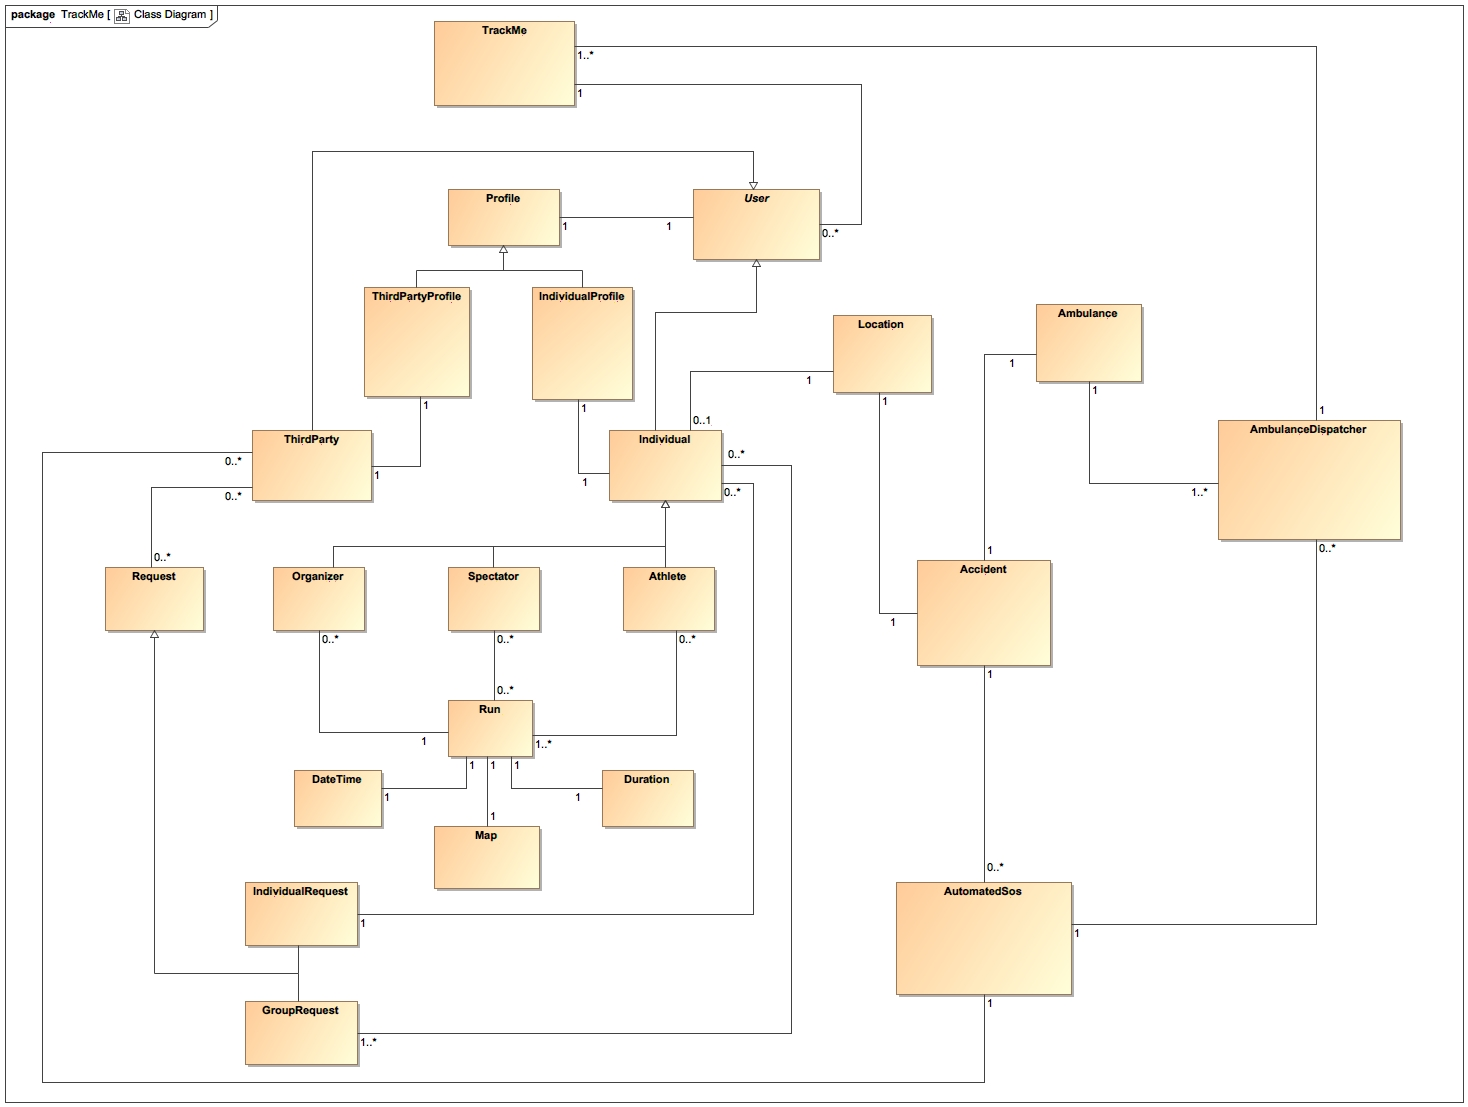
\includegraphics[width=\textwidth]{images/UML/ClassDiagram.jpg}
        \caption{Domain Model}
    \end{figure}
    
    \newpage
    
    \subsubsection{State Charts}
    \begin{figure}[!ht]
        \centering
        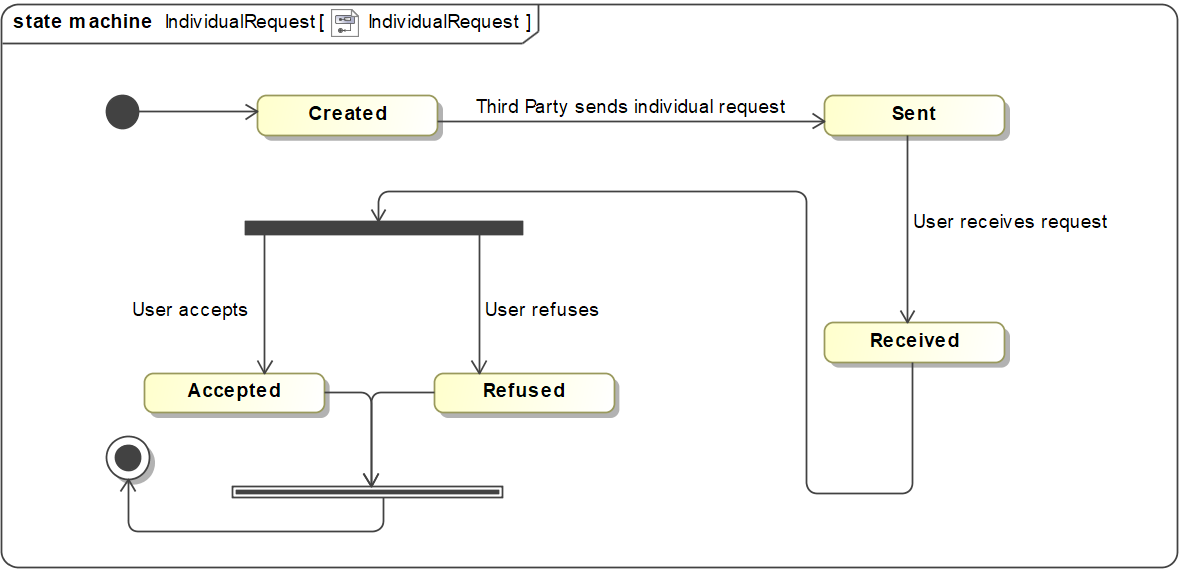
\includegraphics[width=\textwidth, keepaspectratio]{images/UML/state_individualRequest.png}
        \caption{State Chart Individual Request}
        \label{fig:state_individual}
    \end{figure}
    \begin{figure}[!ht]
        \centering
        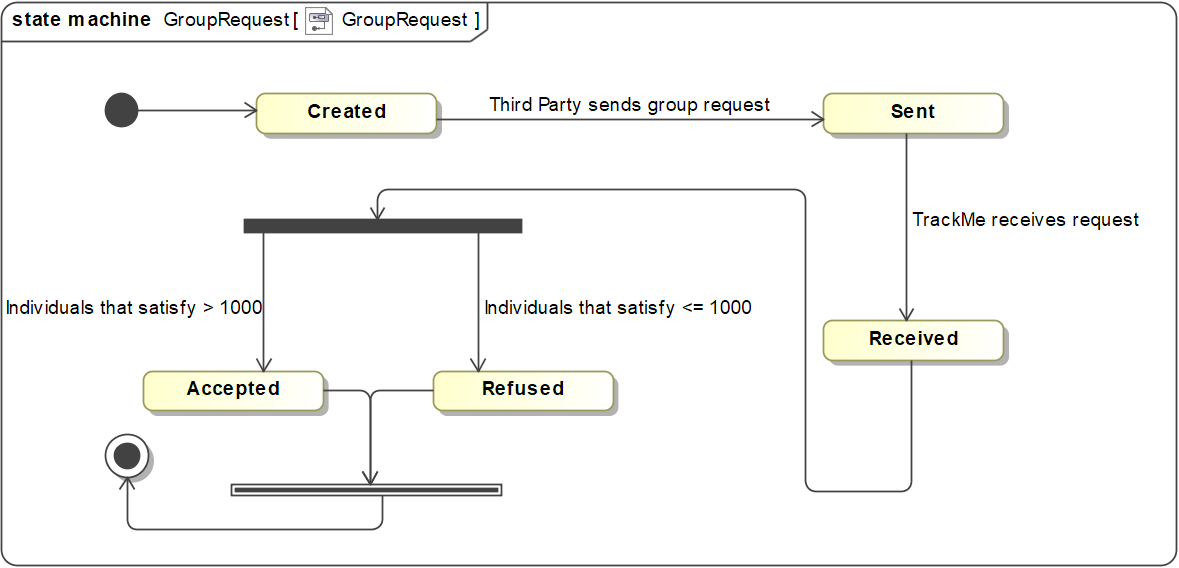
\includegraphics[width=\textwidth, keepaspectratio]{images/UML/state_groupRequest.png}
        \caption{State Chart Group Request}
        \label{fig:state_group}
    \end{figure}
    \begin{figure}[!ht]
        \centering
        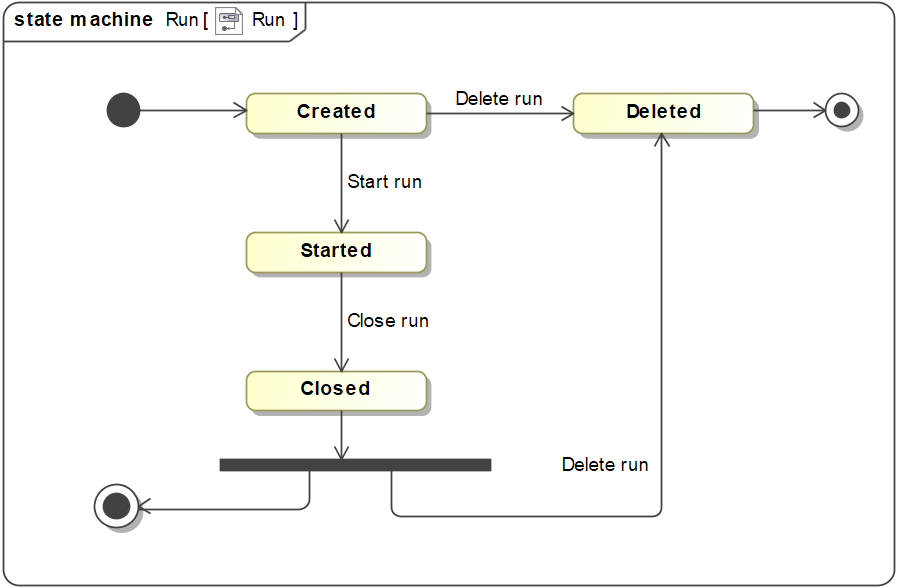
\includegraphics[width=\textwidth, keepaspectratio]{images/UML/state_run.png}
        \caption{State Chart Run}
        \label{fig:state_run}
    \end{figure}
    \newpage

    \subsection{Product Functions}
    \textit{TrackMe} will provide three main services: \textit{Data4Help}, \textit{Automated-SOS} and \textit{Track4Run}.
    
    \paragraph{Data4Help :}
    the application will provide both \textit{"Sign-on"} and \textit{"Sign-in"} pages and will be able to register new users and to check credentials used to login.
    
    To register himself an user must provide an username and a password as well as his personal information. To be logged in, the user should send through the login form his credentials which the system will use to authenticate him.
    
    \textit{TrackMe} may yield an interface that allows individual users to connect external devices and if so, of course a method for acquiring data from it.
    
    The application should also provide to third-parties two possible data request options:
    \begin{itemize}
        \item Individual Data request: sent directly to the individual if they know an  individual by his/her social security number or fiscal code in Italy;
        \item Group Data request: access  to  anonymous  data  of  groups  of  individuals, if \textit{TrackMe}  that  approves  them  if  it  is  able  to  properly  anonymize  the  requested  data.
    \end{itemize}
    
    \paragraph{Automated-SOS:} the system implements \textit{Data4Help} services to manage individual's personal data and provide them to third-parties who requested for. In addition, there should be an interface both for third-party and individual users registered to \textit{Data4Help} that wants to enable an \textit{Automated-SOS} service. This feature should be able to use users' data to monitor their health status and, when such parameters are below certain thresholds, sends the location of the customer to an ambulance. Thus, the application should be able to interact with the GPS system of the customers' devices.
    
    \textit{Automated-SOS} is built on top of \textit{Data4Help} and provides individuals the capability of subscribing to third-parties who has enabled the service.
    
    \paragraph{Track4Run: } the software should provide to users that wants to use \textit{Track4Run} all the facilities they need such as a page for the creation of a new run with all the information (track, date and time) and two different pages to allow both spectators and athletes either watch or enroll/unroll to an existing run.
    
    \textit{Track4Run} is also built on top of \textit{Data4Help} and allows third parties to create new runs where athletes can participate. Athletes' position can be tracked and it will be sent to all spectators that are watching the run on a map.
    
    \subsection{User Characteristics}
        \subsubsection{Data4Help}
        \begin{itemize}
            \item \textbf{Guest:} a customer that is visiting \textit{TrackMe}. He can only login or register to the system.
            \item \textbf{User:} a \textit{Guest} successfully registered to \textit{TrackMe} and logged in to the system. He can be either an \textit{Individual} or a \textit{Third Party.}
            \item \textbf{Individual:} an \textit{User} that agreed that \textit{TrackMe} can collect his personal data. He is identified by a SSN/FC. Data acquisition can happen through smart watches or similar devices.
            \item \textbf{Third Party:} an \textit{User} that can ask an \textit{Individual} to gain access to their personal data. He is identified by a VAT number. He can also request access to data that belongs to a group of \textit{Individuals}, but the request shall be accepted only if \textit{TrackMe} can guarantee anonymity to the requested data. During a request he can also subscribe to new data that will be received as soon as is it is produced.
        \end{itemize}

        \subsubsection{Automated-SOS Extension}
        \begin{itemize}
            \item \textbf{Individual:} he can access to a list of Third Parties that enabled the Automated-SOS service. He can also select a Third Party from the list and subscribe to it.
            \item \textbf{Third Party:} it has the ability to enable the Automated-SOS service so that any Individual can subscribe to it.
        \end{itemize}
        
        \subsubsection{Track4Run Extension}
        \begin{itemize}
            \item \textbf{Organizer:} both an \textit{Individual} and a \textit{Third Party} that created at least one run. He can create, start or delete a run.
            \item \textbf{Athlete:} an \textit{Individual} that enrolled a created run. His position will be sent to all Spectators that joined that run.
            \item \textbf{Spectator:} an \textit{Individual} that joined a started run. He can see the position of all Athletes that are competing in the run until the run is finished.
        \end{itemize}
    
    \subsection{Assumptions and Dependencies}

        \subsubsection{Assumptions}
        \begin{description}
        \item[A-01] The field "Password" and "Repeat Password" match.
        \item[A-02] Data provided by the individual, such as email and SSN, are valid.
        \item[A-03] Data provided by the Third-Party (i.e: VAT number) are valid.
        \item[A-04] The user is already registered.
        \item[A-05] Username and password provided match the ones previously stored in the registration process.
        \item[A-06] The user is logged in the system.
        \item[A-07] The Third-Party provides a SSN/FC of an individual already registered into the system.
        \item[A-08] The Third-Party provides not contradictory criteria for the selection of the group of individuals.
        \item[A-09] The Third-Party has sent at least a request to the user whose data she wants to subscribe.
        \item[A-10] The external device provided by the user is compatible with the system.
        \item[A-11] The user has activated NFC/Bluetooth on the mobile device.
        \item[A-12] The user has activated NFC/Bluetooth on the external device.
        \item[A-13] An Automated-SOS service is enabled from at least one Third Party.
        \item[A-14] At least one ambulance dispatcher is available for SOS request serving.
        \item[A-15] The dispatcher is able to communicate with both the individual and the ambulance associated with the accident.
        \item[A-16] The organizer defines a not empty path.
        \item[A-17] The Organizer has already created a run.
        \item[A-18] At least two athletes are enrolled in the run.
        \item[A-19] There is at least one created run.
        \item[A-20] The Athlete is enrolled to at least one run.
        \item[A-21] There is at least one started run.
        \item[A-22] The individual has approved \textit{TrackMe}'s terms of use.
        \item[A-23] The individual has received at least an individual request.
        \item[A-24] The individual has accepted the individual request.
        \item[A-25] The system can access individual's mobile device position through GPS.
        \item[A-26] Username is not already taken.
        \item[A-27] Password is valid (i.e.: at least 8 alphanumerical characters).
        \item[A-28] The run has not been started.
        \end{description}
        
%%%%%%%%%%%%%%%%%%%%%%%%%%%%%%%%%%%%%%%%%%%%%%%%%%%%%%%%%%%%%%
\newpage
\section{Specific Requirements}

    \subsection{External Interface Requirements}
        
        \subsubsection{User Interfaces}
        
        The mobile application shall provide login and two different registration interfaces for both individual and third parties.
        
        \begin{figure}[!htpb]
    	\centering
    	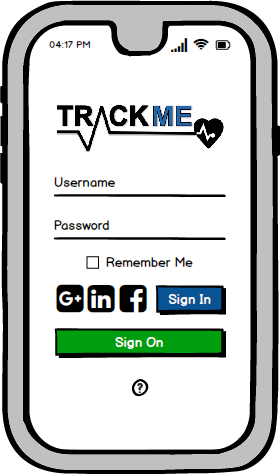
\includegraphics[height=50mm]{images/mockups/Login_Registration.png}
    	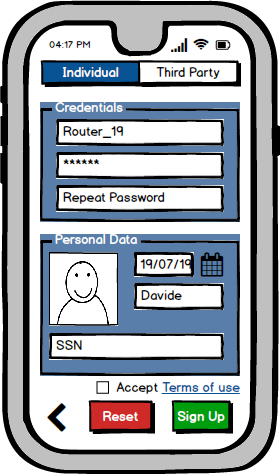
\includegraphics[height=50mm]{images/mockups/RegistrationForm.png}
    	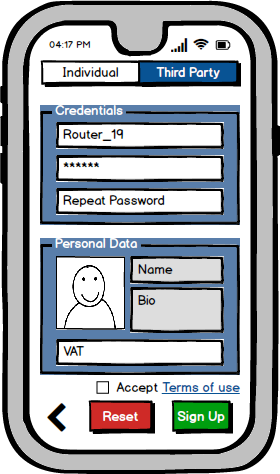
\includegraphics[height=50mm]{images/mockups/ThirdPartyRegistration.png}
        \end{figure}
        
        The users would also be able to manage their profile by swiping left from the home page.
        
        \begin{figure}[!htpb]
    	\centering
    	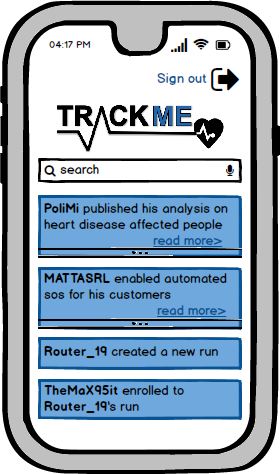
\includegraphics[height=50mm]{images/mockups/HomePage.png}
    	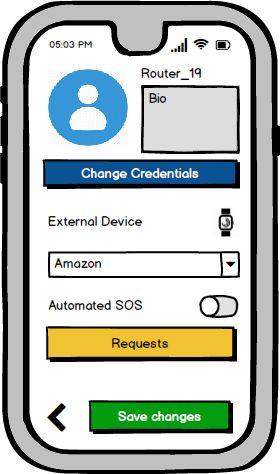
\includegraphics[height=50mm]{images/mockups/IndividualProfile.png}
    	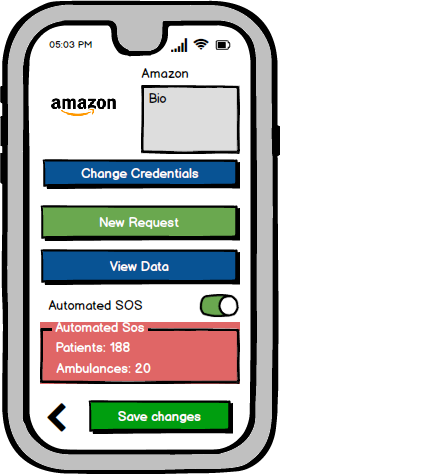
\includegraphics[height=50mm]{images/mockups/ThirdPartyProfile.png}
        \end{figure}
        \newpage
        \textit{TrackMe} shall provide an ease of use management interface for requests handling.
        \begin{figure}[!htpb]
    	\centering
    	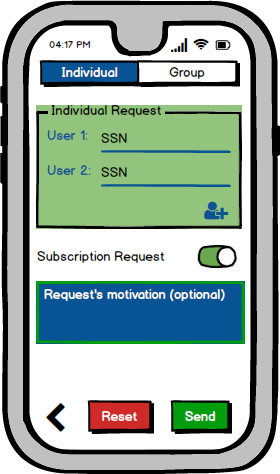
\includegraphics[height=50mm]{images/mockups/Requests.png}
    	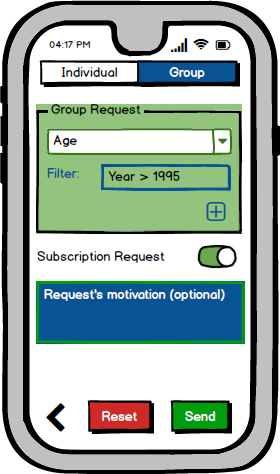
\includegraphics[height=50mm]{images/mockups/GroupRequest.png}
    	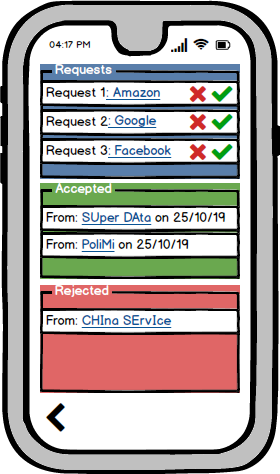
\includegraphics[height=50mm]{images/mockups/ManageRequests.png}
    	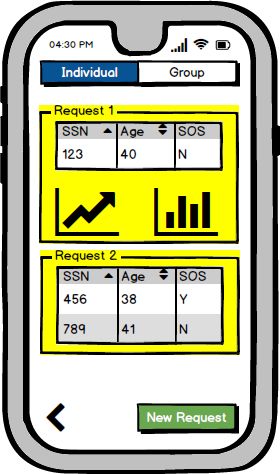
\includegraphics[height=50mm]{images/mockups/ViewData.png}
    	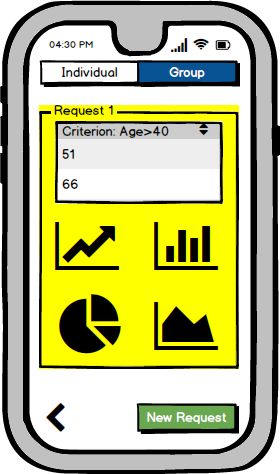
\includegraphics[height=50mm]{images/mockups/ViewData2.png}
        \end{figure}
        
        Instead, swiping right from the home all the \textit{Track4Run} facilities:
        \begin{figure}[!htpb]
    	\centering
    	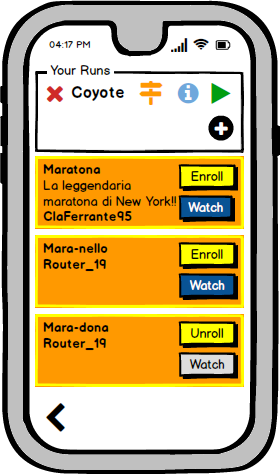
\includegraphics[height=50mm]{images/mockups/RunManager.png}
    	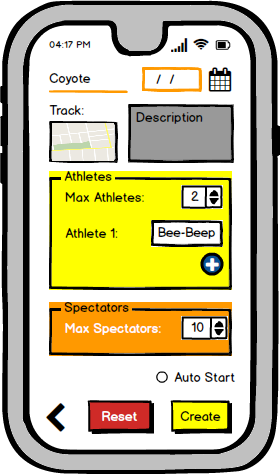
\includegraphics[height=50mm]{images/mockups/RunCreate.png}
    	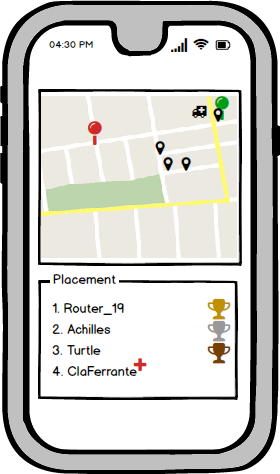
\includegraphics[height=50mm]{images/mockups/ShowMap.png}
    	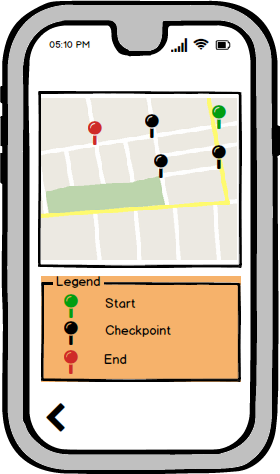
\includegraphics[height=50mm]{images/mockups/DefineTrack.png}
        \end{figure}
        \newpage
        \subsubsection{Hardware Interfaces}
        The GPS system of the smartphone or the one of the external device (if connected) is needed in order to track customer's position.
        
        Furthermore, a separate system to notify the ambulances in case of accident shall be integrated within already existing ambulances' on-board technologies. This system and further interactions with \textit{TrackMe} are out of scope of this specification document.
        
        \subsubsection{Software Interfaces}
        Both the front end and the back-end should be compatible with most of existing PC and mobile operating systems. The mobile and application should indeed be supported at least on Android Lollipop 5.0 and iOS5 or major versions; the web application shall instead be compatible with different browsers such as Google Chrome (with V8 JavaScript engine), Mozilla Firefox v3.0 (or major) and Safari v4.0 (or major).
        
        Moreover the developer could choose to implement REST services to improve portability, reliability, modifiability and simplicity of the software.
        
        \subsubsection{Communication Interfaces}
        The application shall communicate with the back-end server over HTTPS and may enable O-Auth2 authentication protocol for clients. In order to connect and interact with external devices the mobile application shall also support BT and/or NFC.
        
        Moreover, the system shall be able to interact with a DBMS both for for storing and retrieving user data, also in real-time in an Automated-SOS related scenario. In addition, the client application should be able to interact with the back-end service which will indeed be able get client requests, send responses and make data available to clients using lightweight object oriented communication protocols such as JSON or CBOR.

\newpage    \subsection{Functional Requirements}

        \subsubsection{Use Cases Diagrams}
        \begin{figure}[!htpb]
    	\centering
    	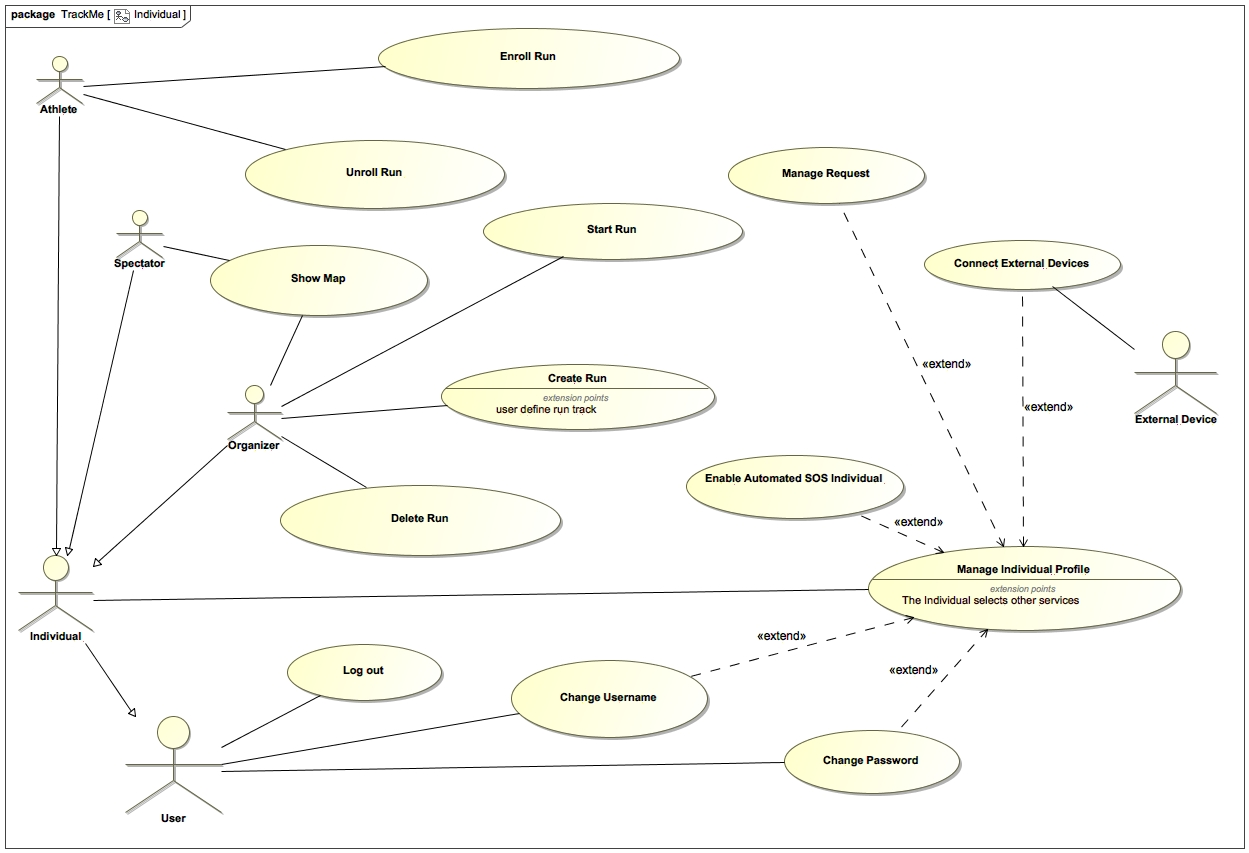
\includegraphics[width=\textwidth]{images/UML/Individual.jpg}
    	\caption{Use Cases: Individual}
    	\end{figure}
    	\begin{figure}[!htpb]
    	\centering
    	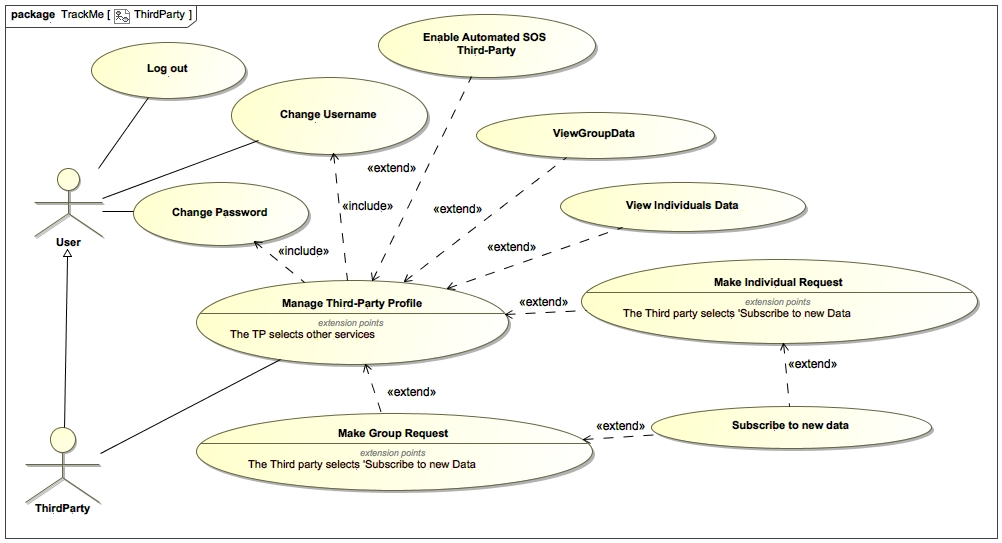
\includegraphics[width=\textwidth]{images/UML/ThirdParty.jpg}
    	\caption{Use Cases: ThirdParty}
        \end{figure}
        \begin{figure}[!htpb]
    	\centering
    	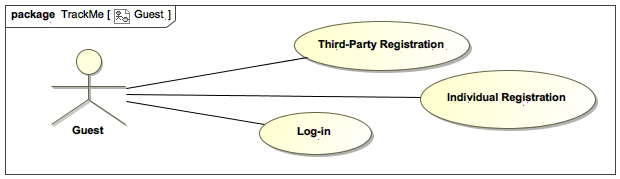
\includegraphics[width=\textwidth]{images/UML/Guest.jpg}
    	\caption{Use Cases: Guest}
    	\end{figure}
    	\begin{figure}[!htpb]
    	\centering
    	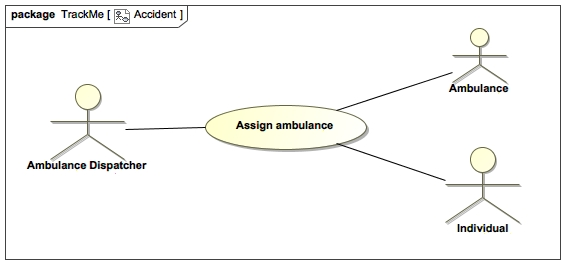
\includegraphics[width=\textwidth]{images/UML/Accident.jpg}
    	\caption{Use Cases: Dispatcher}
    	\end{figure}
        \newpage
        
        
        \subsubsection{Individual Registration}
		\begin{description}
        	\item[GOAL-01] Allow a guest to register as an Individual.
                    \begin{itemize}
            	    \item[\requirement]
                	\begin{description}
                	\item[REQ-01] A customer not signed-on must be able to begin the individual's registration process to \textit{TrackMe} providing a username, a password and his personal data.
                	\end{description}
                	\item
                	\begin{description}
                	\item[A-26] Username is not already taken.
                	\end{description}
                	\item
                	\begin{description}
                	\item[A-27] Password is valid (i.e.: at least 8 alphanumerical characters).
                	\end{description}
                	\item
                	\begin{description}
                	\item[A-01] The field "Password" and "Repeat Password" match.
                	\end{description}
                	\item
                	\begin{description}
                	\item[A-02] Data provided by the individual, such as email and SSN, are valid.
                	\end{description}
                	\item
                	\begin{description}
                	\item[A-22] The guest has approved \textit{TrackMe}'s terms of use
                	\end{description}
                	\end{itemize}
        \end{description} 
        
        \begin{usecase}{Individual  Registration}
        \name{Individual Registration}
        \brief{A guest sign up to the application as an Individual.}
        \actor{Guest.}
        \pre{The individual has a valid SSN/FC and he has selected the \textit{Individual} option in the Registration use case.}
        \bflow{The system asks to provide username, password, SSN/FC (based on region) and user personal information such as name, surname, age, gender, e-mail, nationality and optional notes about his health condition.}
              {The individual fills out the requested information and presses the confirm button.}
              {The system registers that user as an Individual and adds it to the  Database.}
        \post{The individual is successfully registered as an Individual.}
        \except{The guest provide a username already present on the database. In this case an error message is printed out the guest must chose a correct username.}
        {If the password chosen is too short an error message is printed out and the guest must chosen an other one.}
      \end{usecase}
        
        \begin{description}
        	\item[GOAL-02] Allow a guest to register as an Third-Party.
            	\begin{itemize}
            	    \item[\requirement]
                	\begin{description}
                	\item[REQ-02]  A customer not signed-on must be able to begin the individual's registration process to \textit{TrackMe} providing a username, a password and its organization data.
                	\end{description}
                	\item
                	\begin{description}
                	\item[A-26] Username is not already taken.
                	\end{description}
                	\item
                	\begin{description}
                	\item[A-27] Password is valid (i.e.: at least 8 alphanumerical characters).
                	\end{description}
                	\item
                	\begin{description}
                	\item[A-01] The field "Password" and "Repeat Password" match.
                	\end{description}
            	    \item
                	\begin{description}
                	\item[A-03] Data provided by the Third-Party (i.e: VAT number) are valid.
                	\end{description}
                	\item
                	\begin{description}
                	\item[A-22] The guest has approved \textit{TrackMe}'s terms of use
                	\end{description}
                \end{itemize}
        \end{description}
        
        
        \begin{usecase}{Third Party Registration}
        \name{Third Party Registration}
        \brief{A guest sign up to the application as a Third-Party}
        \actor{Guest.}
        \pre{The third party has a valid VAT and he has selected the \textit{Third-Party} option in the Registration use case.}
         \bflow{TrackMe asks to provide a VAT number and organization personal information.}
              {The Third-Party fills out the requested information and presses the confirm button.}
               {TrackMe asks to provide username and password.}
              {The system registers that user as a Third-Party and adds it to the  Database.}
        \post{The individual is successfully registered as a Third-Party.}
        \except{The guest provide a username already present on the database. In this case an error message is printed out the guest must chose a correct username.}
        {If the password chosen is too short an error message is printed out and the guest must chosen an other one.}
      \end{usecase}
        
        
        \subsubsection{Log-in}
        
        
        \begin{description}
        	\item[GOAL-03] The guest should be able to sign in into the application.
            	\begin{itemize}
            	    \item[\requirement]
                	\begin{description}
                	\item[REQ-03] The system must provide a log-in interface for already registered users, not previously signed into the application.
                	\end{description}
                	\item
                	\begin{description}
                	\item[A-04] The user is already registered.
                	\end{description}
                	\item
                	\begin{description}
                	\item[A-05] Username and password provided match the ones previously stored in the registration process.
                	\end{description}
                	\end{itemize}
        \end{description}
        
        
        \begin{usecase}{Log-in}
        \name{Log-in}
        \brief{A Guest sign in to access the application.}
        \actor{Guest.}
        \pre{The Guest is already registered and it's on the main page.}
        \bflow{TrackMe provides to the \textit{Guest} a form composed by two text boxes where the user can write and a button to send the form. The first box is the \textit{'username'}, while the latter is the \textit{'password'} field.}
              {The Guest writes his username on the \textit{'username'} box and his associated password on \textit{'password'} box and presses the Log-in button.}
              {TrackMe checks the username is on the DB and that its associated password is correct. and checks whether he is  registered as individual or Third Party}
              {TrackMe finds that username and its associated password are valid and let the guest log-in into the system.}
        \post{The Guest is successfully authenticated either as Individual or Third-Party.}
        \except{If the username is not present in the database an error message is showed and the access to the system is not granted }
        {If the password inserted is not associated with the given username, an error message is showed and the guest cannot access the system}
        \end{usecase}
        
        
        \subsubsection{Profile Management }
        
        \begin{description}
        	\item[GOAL-04] The user should be able to change his username.
            	\begin{itemize}
            	    \item[\requirement]
                	\begin{description}
                	\item[REQ-04] TrackMe must provide to users the possibility to change their username. 
                	\end{description}
                	\item
                	\begin{description}
                	\item[A-06] The user is logged in the system.
                	\end{description}
                	\item
                	\begin{description}
                	\item[A-26] Username is not already taken.
                	\end{description}
                	\end{itemize}
        \end{description}
        
        
        
       \begin{usecase}{User Changes Username}
        \name{User Changes Username}
        \brief{A user changes his username}
        \actor{User.}
        \pre{The User is logged in the system and is in the change credentials section.}
        \bflow{The User clicks on the  \textit{'Change credentials'} button and select "Username".}
              {The User is redirect to a page and he can now insert a new username writing it into a box}
              {The User clicks on the submit button}
              {The user's row in the database is updated with his new username}
        \post{The has updated his username.}
        \except{The new username is already present on the database and an error mistake is showed}
       \end{usecase}
       
               \begin{description}
        	\item[GOAL-05] The user should be able to change his password.
            	\begin{itemize}
            	    \item[\requirement]
                	\begin{description}
                	\item[REQ-05] TrackMe must provide to registered users the possibility to change their password. 
                	\end{description}
                	\item
                	\begin{description}
                	\item[A-05] Username and password provided match the ones previously stored in the registration process.
                	\end{description}
                	\item
                	\begin{description}
                	\item[A-06] The user is logged in the system.
                	\end{description}
                	\end{itemize}
        \end{description}
       
       
       
       \begin{usecase}{User Changes password}
        \name{User Changes  password}
        \brief{A user changes his password}
        \actor{User.}
        \pre{The User is logged in the system and is in the change credentials section.}
        \bflow{The User clicks on the  \textit{'Change credentials'} button and select "Password".}
              {The system asks to the user to insert the old password, a new password and to repeat the latter once}
              {The User clicks on the submit button}
              {The user's row in the database is updated with his new password}
        \post{The user has changed his password.}
        \except{If the new password is too short and an error message is showed}
        {If the old password inserted is not correct an error message is printed out}
       \end{usecase}
       
        \begin{description}
        	\item[GOAL-06] The user should be able to log-out from the system. 
            	\begin{itemize}
            	    \item[\requirement]
                	\begin{description}
                	\item[REQ-06] The system must provide the possibility to the user of logging out. 
                	\end{description}
                	\item
                	\begin{description}
                	\item[A-06] The user is logged in the system.
                	\end{description}
                	\end{itemize}
        \end{description}
              
       \begin{usecase}{User Log-out}
        \name{User Log-out}
        \brief{A user logs out from the system}
        \actor{User.}
        \pre{The User is logged in the system and is on the main page.}
        \bflow{The User clicks on the  \textit{'Log-out'} button.}
              {The system asks to the user if he is sure he wants to log-out the system}
              {The user confirm}
         \post{The user is not logged anymore into TrackMe}
        \end{usecase}
       
       \begin{description}
        	\item[GOAL-07] The individual should be able to change his personal data. 
            	\begin{itemize}
            	    \item[\requirement]
                	\begin{description}
                	\item[REQ-07] The system must provide the possibility to change Individual's personal data. 
                	\end{description}
                	\item
                	\begin{description}
                	\item[A-02] Data provided by the individual, such as email and SSN, are valid.
                	\end{description}
                	\item
                	\begin{description}
                	\item[A-06] The user is logged in the system.
                	\end{description}
                	\end{itemize}
        \end{description}
      
      
       \begin{usecase}{Manage Individual Profile}
        \name{Manage Individual Profile}
        \brief{An individual can change the setting of his profile}
        \actor{Individual.}
        \pre{The User is logged in the system as an Individual and he's on the profile page.}
        \bflow{The system provides a box with the user's description, and a box with the user's image}
        {\begin{itemize}
            \item The Individual can change any of its personal data.
            \item The user can click on the image to update his picture
        \end{itemize}}
        {The individual clicks on the \textit{Save Changes} button provided by TrackMe}
        \post{The individual has modified his profile data}
        \epoint{The Individual clicks on the\textit{ Manage Request}, \textit{Connects External Devices} or \textit{Enable Automated SOS button}}
       \end{usecase}
       
       \begin{description}
        	\item[GOAL-08] The Third-Party should be able to change his organization data. 
            	\begin{itemize}
            	    \item[\requirement]
                	\begin{description}
                	\item[REQ-08] The system must provide the possibility to change Third Party's organization data. 
                	\end{description}
                	\item
                	\begin{description}
                	\item[A-03] Data provided by the Third-Party (i.e: VAT number) are valid.
                	\end{description}
                	\item
                	\begin{description}
                	\item[A-06] The user is logged in the system.
                	\end{description}
                	\end{itemize}
        \end{description}
       
       \begin{usecase}{Manage Third-Party Profile}
        \name{Manage Third-Party Profile}
         \brief{An Third-Party can change the setting of his profile}
        \actor{Third-Party.}
        \pre{The User is logged in the system as a Third-Party and he's on the profile page.}
        \bflow{The system provides a box with the user's description, and a box with the user's image}
        {\begin{itemize}
            \item The Third-Party can change any of its personal data.
            \item The user can click on the image to update his picture
        \end{itemize}}
        {The Third-Party clicks on the \textit{Save Changes} button provided by TrackMe}
        \post{The Third-Party has modified his profile data}
        \epoint{The Third-Party clicks on one of the following buttons: \textit{Enable Automated SOS }, \textit{Make Individual Request}, \textit{Make Group Request}, \textit{View Data} }
       \end{usecase}
           
           
        \subsubsection{Data4Help}
      
            \begin{description}
        	\item[GOAL-09] The Third-Party should be able to send requests to the individuals. 
            	\begin{itemize}
            	    \item[\requirement]
                	\begin{description}
                	\item[REQ-09] Data4help must allow the Third-Parties to send a request to a particular individual, provided his SSN/FC. 
                	\end{description}
                	\item
                	\begin{description}
                	\item[A-06] The user is logged in the system.
                	\end{description}
                	\item
                	\begin{description}
                	\item[A-07] The Third-Party provides a SSN/FC of an individual already registered into the system.
                	\end{description}
                	\end{itemize}
        \end{description}
      
        \begin{usecase}{ Make Individual Request}
        \name{Make Individual Request}
        \brief{A third party sends a request to an individual to view his data.}
        \actor{Third Party.}
        \pre{The third-party is logged-in, has selected the \textit{'Make Individual Request'} option and has a valid SSN/FC of a registered individual.}
        \bflow{TrackMe provides a box called \textit{'SSN/FC'} where the third party writes the individual \textit{'SSN/FC'}}
        {Third Party presses the \textit{'Submit'} button.}
        {TrackMe sends the data request to the individual and informs the Third-Party user that the operation succeed.}
        \post{The third party has access to the data of the individual who received the request.}
        \epoint{The Third-Party selects the 'Subscribe to new data' option}
        \end{usecase}
        
        \begin{description}
        	\item[GOAL-10] The Third-Party should be able to make group requests. 
            	\begin{itemize}
            	    \item[\requirement]
                	\begin{description}
                	\item[REQ-10] Data4help must allow the Third-Parties to generated a request for a group of individuals. 
                	\end{description}
                	\item[\requirement]
                	\begin{description}
                	\item[REQ-11] The system must be able to anonymize users' requested data. 
                	\end{description}
                	\item
                	\begin{description}
                	\item[A-06] The user is logged in the system.
                	\end{description}
                	\item
                	\begin{description}
                	\item[A-08] The Third-Party provides not contradictory criteria for the selection of the group of individuals.
                	\end{description}
                	\end{itemize}
        \end{description}
        
        \begin{usecase}{Make Group Request}
        \name{Make Group Request}
        \brief{A third party make a group request that allows to see data of a group of individuals .}
        \actor{Third Party.}
        \pre{The third-party is logged-in and has selected the 'Make Group Request' option}
        \bflow{TrackMe provides an interface in which a third-party can insert search criteria for group requests.}
        {Third party fills out the form and then presses the button \textit{'Send Request'}.}
        {TrackMe checks if the number of individuals of the group who matches the search criteria defined on point \textit{a)} is greater than 1000.}
        {TrackMe informs the Third-Party that the operation succeed.}
        \post{The third party has access to the data of a specific group of individuals who received the request.}
        \except{If the number of individual selected is lower than 1000 an error message is printed and the request is denied}
        \end{usecase}
        
                \begin{description}
        	\item[GOAL-11] The Third-Party should be able to subscribe to new data, once an Individual request is made. 
            	\begin{itemize}
            	    \item[\requirement]
                	\begin{description}
                	\item[REQ-12] Data4help must allow the Third-Parties to choose if subscribe to new data associated with a particular Individual. 
                	\end{description}
                	\item[\requirement]
                	\begin{description}
                	\item[REQ-13] The system must be able to periodically query the database in order to get new data as soon as they are produced.
                	\end{description}
                	\item
                	\begin{description}
                	\item[A-06] The user is logged in the system.
                	\end{description}
                	\item
                	\begin{description}
                	\item[A-09] The Third-Party has sent at least a request to the user whose data she wants to subscribe.
                	\end{description}
                	\item
                	\begin{description}
                	\item[A-23] The individual has received at least an individual request.
                	\end{description}
                	\item
                	\begin{description}
                	\item[A-24] The individual has accepted the individual request.
                	\end{description}
                	\end{itemize}
        \end{description}
        
        \begin{usecase}{Subscribe to New Data}
        \name{Subscribe to New Data}
        \brief{A third party subscribes to the data of individuals who received at least a request.}
        \actor{Third Party.}
        \pre{The Third-Party is logged-in and is on requests page.}
        \bflow{TrackMe provides a check-box to allow a third-party to choose if she wants to be subscribed to new data.}
            {Third party checks the \textit{'Subscribe'} box.}
            {TrackMe queries periodically the database to check if data has changed and if so will send the new data to the subscribed third-party.}
        \post{The third party is subscribed to the individuals' data and will receive new data as soon as they are produced.}
        \end{usecase}
        
        \begin{description}
        	\item[GOAL-12] The Individual should be able to accept or reject a request coming from a Third-Party. 
            	\begin{itemize}
            	    \item[\requirement]
                	\begin{description}
                	\item[REQ-14] Data4help must allow the Individual to see a list of the received requests from Third Parties. 
                	\end{description}
                	\item[\requirement]
                	\begin{description}
                	\item[REQ-15] Data4help must allow the Individual to accept or reject a request from the list. 
                	\end{description}
                	\item
                	\begin{description}
                	\item[A-06] The user is logged in the system.
                	\end{description}
                	\item
                	\begin{description}
                	\item[A-23] The individual has received at least an individual request.
                	\end{description}
                	\end{itemize}
        \end{description}
        
        \begin{usecase}{Manage Request}
        \name{Manage Request}
        \brief{An individual accepts the request to view his personal data.}
        \actor{Individual.}
        \pre{The individual is logged-in and has selected  the 'Manage Request' option in the main page.}
        \bflow{TrackMe sends to the individual a request to view his data. The individual can see that the request was sent by a specific third-party. TrackMe provides two buttons called \textit{Accept} and \textit{Reject}.}
              {The individual presses the accept button.}
              {TrackMe sends to the third-party a confirmation about his request for that Individual.}
        \post{The third party has access to the Individual data.}
        \end{usecase}
        
        
        \begin{usecase}{View Data}
        \name{View Data}
        \brief{A Third-Party can view the Data of the Individuals that have accepted its requests.}
        \actor{Third-Party.}
        \pre{The Third-Party is logged-in and Is in the section to see the data collected by the application.}
        \bflow{The system provides a list of all request sent by the Third-Party}
        \post{The Third-Party can observe the Individual data.}
        \end{usecase}
        
        
        
        \subsubsection{Connection of External Devices}

 \begin{description}
        	\item[GOAL-13] The Individual shall be able connect an external device to the system.
            	\begin{itemize}
            	    \item[\requirement]
                	\begin{description}
                	\item[REQ-16] Data4help must allow the Individual to connect an external device through BT or NFC.
                	\end{description}
                	\item
                	\begin{description}
                	\item[A-06] The user is logged in the system.
                	\end{description}
                	\item
                	\begin{description}
                	\item[A-10] The external device provided by the user is compatible with the system.
                	\end{description}
                	\item
                	\begin{description}
                	\item[A-11] The user has activated NFC/Bluetooth on the mobile device.
                	\end{description}
                	\item
                	\begin{description}
                	\item[A-12] The user has activated NFC/Bluetooth on the external device.
                	\end{description}
                	\end{itemize}
        \end{description}.
        
        
        \begin{usecase}{Connect External Device}
        \name{Connect External Device}
        \brief{An Individual can connect External Device that allows the system to collect data.}
        \actor{Individual.}
        \pre{The Individual is logged in and is in the section that allows to connect an external device.}
        \bflow {The system provides two drop-down menus that allows the user specify the type of device and which kind of wireless connection uses: Bluetooth or NFC}
        {The user selects the desired option and checks the type of connection, than presses the \textit{Confirm} button}
        {Track4Run asks now to connect the device in the way previously chosen}
        {The Individual connects the device}
        \post{The system can now collect data from the external device.}
        \end{usecase}
        
        
        
        \subsubsection{Automated-SOS }
        
         \begin{description}
        	\item[GOAL-14] The Third-Party shall be able to activate Automated-SOS service.
            	\begin{itemize}
            	    \item[\requirement]
                	\begin{description}
                	\item[REQ-17] The system must allow the Third-Party to activate Automated-SOS service.
                	\end{description}
                	\item[\requirement]
                	\begin{description}
                	\item[REQ-18] The system must be able to assign an ambulance dispatcher to the SOS service.
                	\end{description}
                	\item
                	\begin{description}
                	\item[A-06] The user is logged in the system.
                	\end{description}
                	\item
                	\begin{description}
                	\item[A-14] At least one ambulance dispatcher is available for SOS request serving.       \end{description}
                	\end{itemize}
        \end{description}.
        
        \begin{usecase}{ Enable Automated-SOS Third Party}
        \name{Enable Automated-SOS Third Party}
        \brief{A Third-Party wants to enable Automated-SOS, a service that guarantees that an ambulance, selected by a dispatcher, will be called in 5 seconds if an individual's health parameters are below certain thresholds. That individual must have enable Automated SOS too.}
        \actor{Third party, Ambulance Dispatcher}
        \pre{The Third-Party is logged-in, it has pressed the Enable Automated SOS on the main page and has not already activate this service.}
        \bflow {Automated-SOS checks if the user has already enabled the service.}
              {Automated-SOS asks if the user wants to enable Automated-SOS. It provides two buttons called \textit{'Confirm'} and \textit{'Back'}.}
              {Third Party presses the \textit{'Confirm'} button.}
              \post{Third-Party has enabled Automated-SOS and individuals that enabled Automated-SOS can see the third-party in the Automated-SOS third-party list. An ambulance dispatcher has been assigned to that Third-Party by the system}
              \except{If no dispatcher is available an error message will be printed out by the system}
        \end{usecase}
  
           \begin{description}
        	\item[GOAL-15] The Individual shall be able to activate Automated-SOS service.
            	\begin{itemize}
            	    \item[\requirement]
                	\begin{description}
                	\item[REQ-19] The system must allow the Individual to activate Automated-SOS service.
                	\end{description}
                	\item[\requirement]
                	\begin{description}
                	\item[REQ-17] The system should allow the Individual to choose between third parties who has enabled the service.
                	\end{description}
                	\item
                	\begin{description}
                	\item[A-06] The user is logged in the system.
                	\end{description}
                	\item
                	\begin{description}
                	\item[A-25] The system can access individual's mobile device position through GPS.
                	\end{description}
                	\end{itemize}
        \end{description}
        
        \begin{usecase}{ Enable Automated-SOS Individual}
        \name{Enable Automated-SOS Individual}
        \brief{An Individual wants to enable Automated-SOS, a service that guarantees that an ambulance, selected by a dispatcher, will be called in 5 seconds if an individual's health parameters are below certain thresholds. The individual will choose the Third-Party that will provide the Automated SOS functionality.}
        \actor{Individual}
        \pre{The Individual is logged-in, it has pressed the Enable Automated SOS on the main page and has not already activate this service.}
        \bflow {Automated-SOS checks if the user has already enabled the service.}
              {Automated-SOS asks if the user wants to enable Automated-SOS. It provides two buttons called \textit{'Confirm'} and \textit{'Back'}.}
              {Individual presses the \textit{'Confirm'} button.}
              {The system provides a table with the list of Third-Parties that have enabled Automated SOS}
              {The users selects a Third-Party desired and presses \textit{Confirm}}
              \post{Individual has enabled Automated-SOS and has selected the Third-Party that will provide that service.}
              \except{If no Third-Parties has activated Automated SOS an error message is printed}
        \end{usecase}
        
         \begin{description}
        	\item[GOAL-16] The Dispatcher shall be able to assign an ambulance to an incident.
            	\begin{itemize}
            	    \item[\requirement]
                	\begin{description}
                	\item[REQ-20] The system must be able to get the Individual position.
                	\end{description}
                	\item[\requirement]
                	\begin{description}
                	\item[REQ-21] The system must be able to send the position to the nearest ambulance.
                	\end{description}
                	\item
                	\begin{description}
                	\item[A-13] An Automated-SOS service is enabled from at least one Third Party.
                	\end{description}
                	\item
                	\begin{description}
                	\item[A-14] At least one ambulance dispatcher is available for SOS request serving \end{description}
                	\item
                	\begin{description}
                	\item[A-15] The dispatcher is able to communicate with both the individual and the ambulance associated with the accident.
                	\end{description}
                	\end{itemize}
        \end{description}
        
        \begin{usecase}{Assign Ambulance}
        \name{Assign Ambulance}
        \brief{The Dispatcher will assign an ambulance to an individual, related to a particular Third-Party, whose actual data has overcame a certain limit.}
        \actor{Ambulance Dispatcher, Ambulance.}
        \pre{At least one ambulance must be available; the Third Party must have enabled Automated-SOS. The individual has selected that Third-Party to provide the service of Automated SOS. The Individual security threshold has been overcame}
        \bflow{The system checks the Individual's health parameters and finds that he has overcame the thresholds.}
              {The ambulance Dispatcher checks in the ambulance database the nearest one available.}
              {Automated-SOS sends to the selected ambulance a request with the GPS position of the subject in danger.}
              {The ambulance selected should accept the request, otherwise Automated-SOS will notify the second ambulance available and so on until the request is accepted.}
        \post{An ambulance will go to the position of the Individual} 
        \end{usecase}
        
        \subsubsection{Track4Run}
        
         \begin{description}
        	\item[GOAL-17] The Organizer shall be able to create a run.
            	\begin{itemize}
            	    \item[\requirement]
                	\begin{description}
                	\item[REQ-22] Track4Run must allow the organizer to create a run with a date, time, duration and a path.
                	\end{description}
                	\item[\requirement]
                	\begin{description}
                	\item[REQ-23] The system must provide an interface that allows the user to define a path on an interactive map.
                	\end{description}
                	\item
                	\begin{description}
                	\item[A-06] The user is logged in the system.
                	\end{description}
                	\item
                	\begin{description}
                	\item[A-17] The organizer defines a not empty path.
                	\end{description}
                	
                	\end{itemize}
        \end{description}
        
         \begin{usecase}{Create Run}
        \name{Create Run}
        \brief{An Individual become an Organizer and creates a new run.}
        \actor{Organizer.}
        \pre{The Individual has clicked on the \textit{Plus} button in the Track4Run section.}
        \bflow{ Track4Run provides a set of boxes called \textit{'Name'}, \textit{'Country'}, \textit{'Date'} \textit{Time} and two buttons called \textit{'Confirm'} and \textit{'Back'}.}
              {The organizer fills the boxes and then presses the \textit('Confirm') button.}
              {Track4Run asks the user to defines a \textit{path} using an interactive map}
              {The Organizer defines the \textit{path} using the tools provided by Track4Run to design a path on the map and presses the \textit{Confirm} button}
              {Track4Run adds the \textit{run} information to the DB.}
              {The system informs the Organizer that the operation succeed.}
        \post{The run is created and has been added to the database and its state is ('created'). The list of available runs is updated}
        \except{If the data and time provided for the run are previous the current one an error message is printed}
        \end{usecase}
        
        
        \begin{description}
        	\item[GOAL-18] The Organizer should be able to start a run.
            	\begin{itemize}
            	    \item[\requirement]
                	\begin{description}
                	\item[REQ-24] Track4Run must allow the organizer to start a run previously created.
                	\end{description}
                	\item
                	\begin{description}
                	\item[A-06] The user is logged in the system.
                	\end{description}
                	\item
                	\begin{description}
                	\item[A-17] The Organizer has already created a run.  
                	\end{description}
                	\item
                	\begin{description}
                	\item[A-18] At least two athletes are enrolled in the run.
                	\end{description}
                	\end{itemize}
        \end{description}
        
        
        \begin{usecase}{Start Run}
        \name{Start Run}
        \brief{An Organizer starts a run that he has previously created.}
        \actor{Organizer.}
        \pre{The Organizer is logged-in and is in the Track4Run section. The run he want to start must have at least two athletes enrolled.}
        \bflow{Track4Run provides a list of runs that the Organizer has created. Furthermore, the system provides two buttons  near the each run: \textit{Play} and \textit{Cross}}
              {Organizer Presses the \textit{Play} button near the run he wants to start.}
              {The system asks the Organizer to confirm his choice}
              {The Organizer clicks on the \textit{start} button}
        \post{The selected run state is now \textit{started} and Athletes and Spectator will be notified.}
        \end{usecase}
        
        \begin{description}
        	\item[GOAL-19] The Organizer should be able to delete a run.
            	\begin{itemize}
            	    \item[\requirement]
                	\begin{description}
                	\item[REQ-25] Track4Run must allow the organizer to delete a run previously created.
                	\end{description}
                	\item
                	\begin{description}
                	\item[A-06] The user is logged in the system.
                	\end{description}
                	\item
                	\begin{description}
                	\item[A-17] The Organizer has already created a run.
                	\end{description}
                	\item
                	\begin{description}
                	\item[A-28] The run has not been started.
                	\end{description}
                	\end{itemize}
        \end{description}
        
        \begin{usecase}{Delete Run}
        \name{Delete Run}
        \brief{An Organizer deletes run that he has previously created.}
        \actor{Organizer.}
        \pre{The Organizer is logged-in and is in the Track4Run section. At least one run has been created}
        \bflow{Track4Run provides a list of runs that the Organizer has created. Moreover, the system provides two buttons \textit{Cross} and \textit{Play}.}
              {Organizer select a \textit{created} run and presses the \textit{'Cross '} button.}
              {The system asks if the Organizer wants to delete the run, and provides two buttons \textit{yes} and \textit{no}}
              {The Organizer clicks on the \textit{yes} button}
        \post{Any Athlete that was subscribed to that run is no longer subscribed. Athletes can no longer subscribe to that run. That run is deleted from the list of available runs.}
        \end{usecase}
        
       \begin{description}
        	\item[GOAL-20] The Athlete should be able to enroll a run.
            	\begin{itemize}
            	    \item[\requirement]
                	\begin{description}
                	\item[REQ-26] Track4Run must allow the Athlete to enroll to an already existing run.
                	\end{description}
                	\item
                	\begin{description}
                	\item[A-06] The user is logged in the system.
                	\end{description}
                	\item
                	\begin{description}
                	\item[A-19] There is at least one created run.
                	\end{description}
                	\end{itemize}
        \end{description}
            
        \begin{usecase}{Enroll a Run}
        \name{Enroll a Run}
        \brief{The Athlete is logged-in and is in the Track4Run section. At least one run has been created}
        \actor{Athlete.}
        \pre{The Athlete is logged-in and is in the Track4Run section. At least one run has been created}
        \bflow{Track4Run provides a list of runs that the user can select. these runs must have the state \textit{not-started}. Track4Run also provides two buttons near each created run:  \textit{'Enroll'}  and  \textit{'Watch'} .}
              { The Individual clicks the \textit{'Enroll'} button of the chosen run.}
              {Track4Run informs the Athlete that the operation succeed.}
        \post{The Athlete successfully enrolls the run and his position will be sent to all \textit{Spectators} that spectate that run.}
        \end{usecase}
        
        \begin{description}
        	\item[GOAL-21] The Athlete should be able to unroll a run.
            	\begin{itemize}
            	    \item[\requirement]
                	\begin{description}
                	\item[REQ-26] Track4Run must allow the Athlete to unroll a run.
                	\end{description}
                	\item
                	\begin{description}
                	\item[A-06] The user is logged in the system.
                	\end{description}
                	\item
                	\begin{description}
                	\item[A-20] The Athlete is enrolled to at least one run.
                	\end{description}
                	\end{itemize}
        \end{description}
        
        \begin{usecase}{Unroll a Run}
        \name{Unroll a Run}
        \brief{An Athlete Unrolls to a run previously enrolled.}
        \actor{Athlete.}
        \pre{The Athlete is logged-in and is in the Track4Run section. He is also enrolled to at least one run.}
        \bflow{Track4Run provides the list of runs to which the athlete is enrolled.  Near each created run the buttons  \textit{'Unroll'}  and  \textit{'Watch'} .}
              {Individual selects one run from the list and presses the \textit{'Unroll'} button.}
              {Track4Run informs the Athlete that the operation succeed.}
        \post{The Athlete is no longer enrolled that run.}
        \end{usecase}
        
        \begin{description}
        	\item[GOAL-22] The Spectator shall be able to watch a run.
            	\begin{itemize}
            	    \item[\requirement]
                	\begin{description}
                	\item[REQ-26] Track4Run must allow the Spectator to see the position of the Athletes on a map during a run.
                	\end{description}
                	\item
                	\begin{description}
                	\item[A-7] The user is logged in the system.
                	\end{description}
                	\item
                	\begin{description}
                	\item[A-21] There is at least one started run.
                	\end{description}
                	\item
                	\begin{description}
                	\item[A-25] The system can access individual's mobile device position through GPS.
                	\end{description}
                	\end{itemize}
        \end{description}

        \begin{usecase}{Watch Run}
        \name{Watch Run}
        \brief{A Spectator wants to watch a \textit{run}.}
        \actor{Spectator.}
        \pre{The Spectators is logged-in and is in the Track4Run section. At least one run has been \textit{Started}.}
        \bflow{Track4Run provides a list of runs with state started the state \textit{started}. Track4Run also provides two buttons: a \textit{Watch} and \textit{Enroll}.}
              {Individual selects one run from the list and presses the \textit{'Watch'} button.}
              {Track4Run now recognize the Individual as a Spectator and shows to him a map with all athletes positions.}
        \post{The Spectator successfully spectates the run.}
        \end{usecase}
        
        \subsection{Design and Implementation Constraints}
    
        \subsubsection{Regulatory Policies}
        In order to grant individual privacy and data anonymity, the system should be able to manage both individual and group requests:
        \begin{itemize}
            \item in case of individual requests, the system shall check that the third-party knows individual's security social number and should guarantee that only trusted third-parties can access his data and,
            \item in case of group requests, \textit{TrackMe} should be able to check in the number of individuals which will receive the request will be greater enough to guarantee user privacy.
        \end{itemize}
        
        \subsection{Software System Attributes}
        \subsubsection{Usability}
        The software application shall be usable for all people including elder ones and not \textit{computers} or \textit{smart-things} experts. Ease of use of both the mobile and the web application are (strictly) needed.
        
        \subsubsection{Reliability}
        The system should work without failures in 99,99\% of the cases. The possibility of a breakdown depends on the stability of the Internet connection and on the availability of the external services such as the Ambulance Dispatcher. In this case the users wont be able to access the system and, in case of accident, no ambulance will receive a call and the user must be informed that the service is unavailable. In case of failure the mean time to repair should be a reasonable time, for example less than 3 days.
       
        \subsubsection{Availability}
        To guarantee the maximum profit by the service, in particular the one provide by Automated-SOS, the system must be available 24 hours per day and 7 day per week; availability shall also be granted by at least one "ambulance dispatcher". For the two other features \textit{Data4Help} and \textit{Track4Run}, small deviations from this requirement will be acceptable.
        
        \subsubsection{Security}
        The user allows the system to collect their health data. Furthermore, the position of the user is also present in the system, to provide services such as Automated SOS an Track4Run. If there is a leak of information the privacy of the user is compromised. For this reason at least these security features shall be granted:
       
        \begin{itemize}
        \item         The users passwords are stored in the database hashed with SHA-256\item       The  connection between the client and server is encrypted and sent over SSL to guarantee integrity of data. 
        \end{itemize}
        \subsubsection{Maintainability}

        The system is backed up 2 times a  week, in order to guarantee the database integrity and consistency. To avoid loss of data  the database is saved in at least two copies and the power supply is provided by a particular system that keeps online at least one database. Moreover, an UPS for each \textit{Data Center} shall be present.
        \subsubsection{Portability}

        The system can work both on smart phone and desktop environment. Any personal computer with Java SDK installed can execute TrackMe server. Different version of Android and iOS can should support the front-end application.

        The developers shall consider that the \textit{E-Health} applications area is a wide and promising market slice thus, in order to be competitive, they should guarantee an high level portability through interactions with other existing widely used software applications and hardware interfaces.
        
        \subsubsection{Performances Requirements}
        
        In case of accident, the application should be able to get users' position and send it to the ambulance dispatcher in reasonable time, then the dispatcher will forward the position to the nearest ambulance; all in less than five seconds.
%%%%%%%%%%%%%%%%%%%%%%%%%%%%%%%%%%%%%%%%%%%%%%%%%%%%%%%%%%%%%%
\newpage
\section{Formal Analysis using Alloy}
\renewcommand*{\lstlistlistingname}{Alloy model samples}
\lstlistoflistings
%definition of alloy language for Latex
\lstdefinelanguage{Alloy}{
	morekeywords={
		module, open, as,
		private, abstract, sig, extends, in,
		lone, some, one, disj,
		fact, pred, fun, assert,
		run, check,
		for, but, exactly,
		this, not, implies, else, let,
		not, no, set, all, sum,
		iff, or, Int, and,
		none, univ, iden,
	},
	sensitive=true,
	morecomment=[l]{//},
	morecomment=[l]{--},
	morecomment=[s]{/*}{*/},
	morestring=[b]{"},
	literate={->}{${\rightarrow}$}1
	% replacing characters can cause problems when copying from PDF to editor
}[keywords,comments,strings]
\lstset {
    language=Alloy,
    frame=tb,
    breaklines=true,
    tabsize=3,
    showstringspaces=false,
    numbers=none,
    commentstyle=\color{commentgreen},
    keywordstyle=\color{blue},
    stringstyle=\color{red},
    basicstyle=\small\ttfamily, % basic font setting
    % keyword highlighting
    classoffset=1, % starting new class
    keywordstyle=\color{weborange},
    classoffset=0,
}
\subsection{Signatures}
    \lstinputlisting[language=Alloy, caption=Data4Help model definition, firstline=0, lastline=38]{TrackMeAlloyModel.als}
    
    \lstinputlisting[language=Alloy, caption=Automated-SOS model definition, firstline=39, lastline=48]{TrackMeAlloyModel.als}
    
    \lstinputlisting[language=Alloy, caption=Track4Run model definition, firstline=49, lastline=78]{TrackMeAlloyModel.als}
    
    \newpage
\subsection{Facts}
    \lstinputlisting[language=Alloy, caption=Common facts, firstline=79, lastline=87]{TrackMeAlloyModel.als}
    
    \lstinputlisting[language=Alloy, caption=Data4Help facts, firstline=88, lastline=115]{TrackMeAlloyModel.als}
    
    \lstinputlisting[language=Alloy, caption=Automated-SOS facts, firstline=116, lastline=137]{TrackMeAlloyModel.als}
    
    \lstinputlisting[language=Alloy, caption=Track4Run facts, firstline=138, lastline=179]{TrackMeAlloyModel.als}
    
    \newpage
\subsection{Predicates}

    \lstinputlisting[language=Alloy, caption=Data4Help predicates, firstline=180, lastline=199]{TrackMeAlloyModel.als}
    
    \lstinputlisting[language=Alloy, caption=Automated-SOS predicates, firstline=200, lastline=209]{TrackMeAlloyModel.als}
    
    \lstinputlisting[language=Alloy, caption=Track4Run predicates, firstline=210, lastline=239]{TrackMeAlloyModel.als}
    
    \lstinputlisting[language=Alloy, caption=Common predicates, firstline=240, lastline=283]{TrackMeAlloyModel.als}
    
    \newpage
\subsection{Worlds}
    \lstinputlisting[language=Alloy, caption=Run data4Help, firstline=284, lastline=284]{TrackMeAlloyModel.als}
    \begin{figure}[!ht]
    	\centering
    	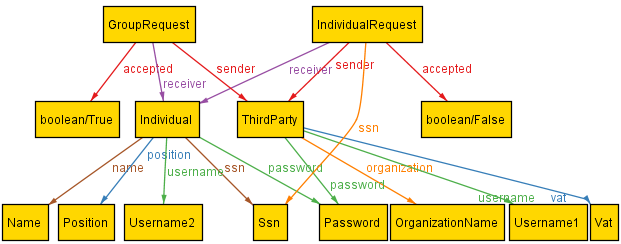
\includegraphics[width=\textwidth]{RASD/images/alloy/data4Help.png}
    \end{figure}
    
    \lstinputlisting[language=Alloy, caption=Run automatedSos, firstline=285, lastline=285]{TrackMeAlloyModel.als}
    \begin{figure}[!ht]
    	\centering
    	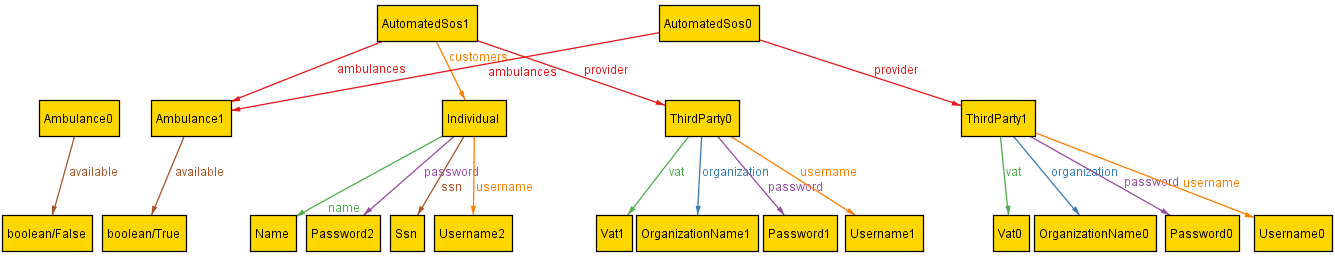
\includegraphics[width=\textwidth]{RASD/images/alloy/automatedSOS.png}
    \end{figure}
    \lstinputlisting[language=Alloy, caption=Run track4Run, firstline=286, lastline=286]{TrackMeAlloyModel.als}
    \begin{figure}[!ht]
    	\centering
    	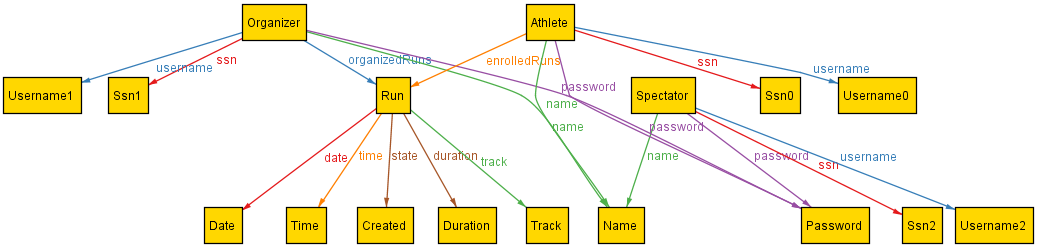
\includegraphics[width=\textwidth]{RASD/images/alloy/track4Run.png}
    \end{figure}
    \newpage
    \lstinputlisting[language=Alloy, caption=Run showAll, firstline=287, lastline=287]{TrackMeAlloyModel.als}
    \begin{figure}[!ht]
    	\centering
    	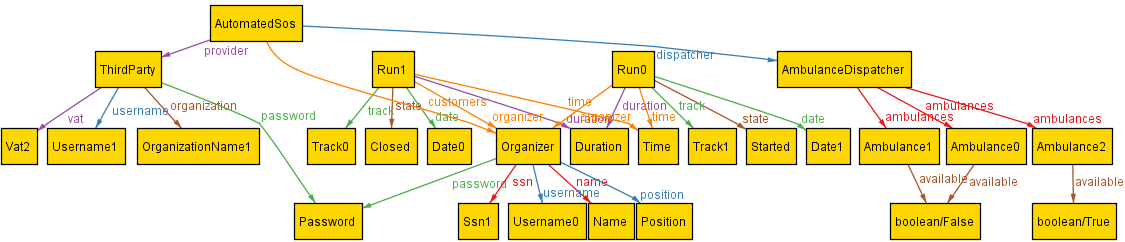
\includegraphics[width=0.91\paperwidth, angle=90]{RASD/images/alloy/showAll.png}
    \end{figure}
    \newpage
%%%%%%%%%%%%%%%%%%%%%%%%%%%%%%%%%%%%%%%%%%%%%%%%%%%%%%%%%%%%%%
\section{Effort Spent}
    \begin{itemize}
        \item[-] \textbf{Davide Rutigliano:}
        
        \item[-] \textbf{Davide Matta:}
        
        \item[-] \textbf{Claudio Ferrante:}
    \end{itemize}

\end{document}